%%---------------Appendices--------------------------------
\appendix
\section*{Appendix A}
\subsection*{Code for API Call}
\begin{lstlisting}[language=R,breaklines]
NJ.2007.2008 <- fromJSON(file = "https://statsapi.web.nhl.com/api/v1/teams/1/stats?season=20072008")
\end{lstlisting} 
\section*{Appendix B}
\subsection*{Uncleaned Data} \small
\begin{verbatim}
> NJ.2007.2008
$copyright
[1] "NHL and the NHL Shield are registered trademarks of the National Hockey League. NHL and NHL team marks are the property of the NHL and its teams. © NHL 2018. All Rights Reserved."
$stats
$stats[[1]]
$stats[[1]]$type
$stats[[1]]$type$displayName
[1] "statsSingleSeason"
$stats[[1]]$splits
$stats[[1]]$splits[[1]]
$stats[[1]]$splits[[1]]$stat
$stats[[1]]$splits[[1]]$stat$gamesPlayed
[1] 82
$stats[[1]]$splits[[1]]$stat$wins
[1] 46
$stats[[1]]$splits[[1]]$stat$losses
[1] 29
$stats[[1]]$splits[[1]]$stat$ot
[1] 7
$stats[[1]]$splits[[1]]$stat$pts
[1] 99
$stats[[1]]$splits[[1]]$stat$ptPctg
[1] "60.4"
$stats[[1]]$splits[[1]]$stat$goalsPerGame
[1] 2.415
$stats[[1]]$splits[[1]]$stat$goalsAgainstPerGame
[1] 2.354
$stats[[1]]$splits[[1]]$stat$evGGARatio
[1] 1.0246
$stats[[1]]$splits[[1]]$stat$powerPlayPercentage
[1] "15.6"
$stats[[1]]$splits[[1]]$stat$powerPlayGoals
[1] 50
$stats[[1]]$splits[[1]]$stat$powerPlayGoalsAgainst
[1] 54
$stats[[1]]$splits[[1]]$stat$powerPlayOpportunities
[1] 320
$stats[[1]]$splits[[1]]$stat$penaltyKillPercentage
[1] "82.8"
$stats[[1]]$splits[[1]]$stat$shotsPerGame
[1] 28.8049
$stats[[1]]$splits[[1]]$stat$shotsAllowed
[1] 27.5244
$stats[[1]]$splits[[1]]$stat$winScoreFirst
[1] 0.725
$stats[[1]]$splits[[1]]$stat$winOppScoreFirst
[1] 0.405
$stats[[1]]$splits[[1]]$stat$winLeadFirstPer
[1] 0.806
$stats[[1]]$splits[[1]]$stat$winLeadSecondPer
[1] 0.879
$stats[[1]]$splits[[1]]$stat$winOutshootOpp
[1] 0.609
$stats[[1]]$splits[[1]]$stat$winOutshotByOpp
[1] 0.514
$stats[[1]]$splits[[1]]$stat$faceOffsTaken
[1] 4286
$stats[[1]]$splits[[1]]$stat$faceOffsWon
[1] 2160
$stats[[1]]$splits[[1]]$stat$faceOffsLost
[1] 2126
$stats[[1]]$splits[[1]]$stat$faceOffWinPercentage
[1] "50.4"
$stats[[1]]$splits[[1]]$stat$shootingPctg
[1] 8.4
$stats[[1]]$splits[[1]]$stat$savePctg
[1] 0.914
$stats[[1]]$splits[[1]]$team
$stats[[1]]$splits[[1]]$team$id
[1] 1
$stats[[1]]$splits[[1]]$team$name
[1] "New Jersey Devils"
$stats[[1]]$splits[[1]]$team$link
[1] "/api/v1/teams/1"
$stats[[2]]
$stats[[2]]$type
$stats[[2]]$type$displayName
[1] "regularSeasonStatRankings"
$stats[[2]]$splits
$stats[[2]]$splits[[1]]
$stats[[2]]$splits[[1]]$stat
$stats[[2]]$splits[[1]]$stat$wins
[1] "6th"
$stats[[2]]$splits[[1]]$stat$losses
[1] "8th"
$stats[[2]]$splits[[1]]$stat$ot
[1] "24th"
$stats[[2]]$splits[[1]]$stat$pts
[1] "6th"
$stats[[2]]$splits[[1]]$stat$ptPctg
[1] "6th"
$stats[[2]]$splits[[1]]$stat$goalsPerGame
[1] "27th"
$stats[[2]]$splits[[1]]$stat$goalsAgainstPerGame
[1] "5th"
$stats[[2]]$splits[[1]]$stat$evGGARatio
[1] "16th"
$stats[[2]]$splits[[1]]$stat$powerPlayPercentage
[1] "25th"
$stats[[2]]$splits[[1]]$stat$powerPlayGoals
[1] "27th"
$stats[[2]]$splits[[1]]$stat$powerPlayGoalsAgainst
[1] "6th"
$stats[[2]]$splits[[1]]$stat$powerPlayOpportunities
[1] "26th"
$stats[[2]]$splits[[1]]$stat$penaltyKillOpportunities
[1] "5th"
$stats[[2]]$splits[[1]]$stat$penaltyKillPercentage
[1] "13th"
$stats[[2]]$splits[[1]]$stat$shotsPerGame
[1] "15th"
$stats[[2]]$splits[[1]]$stat$shotsAllowed
[1] "8th"
$stats[[2]]$splits[[1]]$stat$winScoreFirst
[1] "13th"
$stats[[2]]$splits[[1]]$stat$winOppScoreFirst
[1] "4th"
$stats[[2]]$splits[[1]]$stat$winLeadFirstPer
[1] "5th"
$stats[[2]]$splits[[1]]$stat$winLeadSecondPer
[1] "14th"
$stats[[2]]$splits[[1]]$stat$winOutshootOpp
[1] "7th"
$stats[[2]]$splits[[1]]$stat$winOutshotByOpp
[1] "7th"
$stats[[2]]$splits[[1]]$stat$faceOffsTaken
[1] "29th"
$stats[[2]]$splits[[1]]$stat$faceOffsWon
[1] "29th"
$stats[[2]]$splits[[1]]$stat$faceOffsLost
[1] "4th"
$stats[[2]]$splits[[1]]$stat$faceOffWinPercentage
[1] "13th"
$stats[[2]]$splits[[1]]$stat$savePctRank
[1] "6th"
$stats[[2]]$splits[[1]]$stat$shootingPctRank
[1] "25th"
$stats[[2]]$splits[[1]]$team
$stats[[2]]$splits[[1]]$team$id
[1] 1
$stats[[2]]$splits[[1]]$team$name
[1] "New Jersey Devils"
$stats[[2]]$splits[[1]]$team$link
[1] "/api/v1/teams/1"
\end{verbatim}
\section*{Appendix C}
\subsection*{Code for Cleaning Data} \small
\begin{verbatim}
NJ.2007.2008 <- NJ.2007.2008$stats[[1]]$splits[[1]]$stat
\end{verbatim}
\subsection*{Cleaned Data}
\begin{verbatim}
> NJ.2007.2008
$gamesPlayed
[1] 82
$wins
[1] 46
$losses
[1] 29
$ot
[1] 7
$pts
[1] 99
$ptPctg
[1] "60.4"
$goalsPerGame
[1] 2.415
$goalsAgainstPerGame
[1] 2.354
$evGGARatio
[1] 1.0246
$powerPlayPercentage
[1] "15.6"
$powerPlayGoals
[1] 50
$powerPlayGoalsAgainst
[1] 54
$powerPlayOpportunities
[1] 320
$penaltyKillPercentage
[1] "82.8"
$shotsPerGame
[1] 28.8049
$shotsAllowed
[1] 27.5244
$winScoreFirst
[1] 0.725
$winOppScoreFirst
[1] 0.405
$winLeadFirstPer
[1] 0.806
$winLeadSecondPer
[1] 0.879
$winOutshootOpp
[1] 0.609
$winOutshotByOpp
[1] 0.514
$faceOffsTaken
[1] 4286
$faceOffsWon
[1] 2160
$faceOffsLost
[1] 2126
$faceOffWinPercentage
[1] "50.4"
$shootingPctg
[1] 8.4
$savePctg
[1] 0.914
\end{verbatim}
\section*{Appendix D}
\newpage
\subsection*{Heat Map} 
\begin{figure}
	\centering
	\includegraphics[width=0.7\linewidth]{"Heat Map"}
	\caption{}
	\label{fig:heat-map}
\end{figure}
\section*{Appendix E}
\subsection*{Error Table}
\begin{longtable}{|c|c|c|c|c|}
	\hline
	Team & Actual Points & $|AIC Error|$ & $|R^2 Error|$ & $|Ridge Error|$ \\
	\hline
	ANA &    101 & 0.24715641 & 1.6061406 & 1.93811452 \\
	ARI &     70 & 0.04901625 & 3.1156016 & 1.28011995 \\
	BOS &    112 & 1.22076767 & 0.1551671 & 0.35062443 \\
	BUF &     62 & 0.65149248 & 0.3898144 & 1.93565395 \\
	CGY &     84 & 0.10388349 & 2.5008741 & 0.82366131 \\
	CAR &     83 & 4.35082331 & 6.4428237 & 3.34184350 \\
	CHI &    76 & 0.55805277 & 1.5191952 & 1.87248740 \\
	\hline
	COL &     95 & 2.07595120 & 3.5134566 & 0.42377953 \\
	CBJ &     97 & 0.54118090 & 2.3700857 & 0.40203955 \\
	DAL &    92  & 3.47583721 & 3.5531989 & 3.01541779 \\
	DET &    73 & 2.20990543 & 4.1350665 & 0.05910152 \\
	EDM &    78 & 0.45954586 & 3.6595266 & 2.39590021 \\
	FLA &    96 & 3.63236821 & 1.4277339 & 2.55620918 \\
	LAK &    98 & 5.80054208 & 4.0342055 & 5.62925663 \\
	MIN &   101 & 0.85378174 & 0.8281129 & 1.44090552 \\
	MON & 71 & 0.74507075 & 1.3535107 & 1.73986889 \\
	NAS &   117 & 4.38299534 & 6.5608927 & 6.24530799 \\
	NJD &    97 & 2.79598870 & 0.2648046 & 2.50731256 \\
	NYR &    80 & 2.04603762 & 0.2853365 & 0.68078794 \\
	NYI &    77 & 0.25901951 & 2.7849972 & 3.14971673 \\
	OTT &    67 & 1.38637441 & 3.2626904 & 3.14999867 \\
	PHI &   98  & 2.13773068 & 3.9597064 & 2.57759596 \\
	PIT &   100 & 0.11463457 & 1.0504457 & 0.27550942 \\
	SJS &   100 & 0.79300290 & 0.8822942 & 0.61392558 \\
	STL &    94 & 1.36968826 & 0.6159767 & 0.76033569 \\
	TBL &   113 & 1.26412616 & 3.0261860 & 0.26612309 \\
	TOR &  105  & 0.89029297 & 3.4357766 & 0.81191281 \\
	VAN &    73 & 1.11990454 & 0.8329045 & 3.84934906 \\
	VGK &   105 & 0.72077358 & 5.7287411 & 0.25785441 \\
	WIN &   114 & 2.61239679 & 3.9654460 & 2.99759161 \\
	\hline
	WSH &   109 & 0.24877122 & 0.7015060 & 2.12668772 \\
	\hline
\end{longtable}
\section*{Appendix F}
\subsection*{R Code}\tiny
\begin{verbatim}
# This library allows us to run logistic regression models
library(glmnet)
# This line reads all of the csv files into R that we are going to use as our data to create the models
Dataset<-(lapply(list.files(), read.csv))
# This line reads in the 2017-2018 data
TrainingSet <- (lapply(list.files(), read.csv))
# These lines clean the dataset
for(i in 1:270){
Dataset[[i]]$X <- NULL
Dataset[[i]]$gamesPlayed <- NULL
}
for(i in 1:31){
TrainingSet[[i]]$X <- NULL
TrainingSet[[i]]$gamesPlayed <- NULL
}
wins <- NULL
losses <- NULL
ot <- NULL
pts <- NULL
ptPctg <- NULL
goalsPerGame <- NULL
goalsAgainstPerGame <- NULL
evGAARatio <- NULL
powerPlayPercentage <- NULL
powerPlayGoals <- NULL
powerPlayGoalsAgainst <- NULL 
powerPlayOpportunities <- NULL
penaltyKillPercentage <- NULL
shotsPerGame <- NULL
shotsAllowed <- NULL
winScoreFirst <- NULL
winOppScoreFirst <- NULL
winLeadFirstPer <- NULL
winLeadSecondPer <- NULL
winOutshootOpp <- NULL
winOutshotByOpp <- NULL
faceOffsTaken <- NULL
faceOffsWon <- NULL
faceOffsLost <- NULL
faceOffWinPercentage <- NULL
shootingPctg <- NULL
savePctg <- NULL

for(i in 1:270){
wins[i] <- Dataset[[i]]$wins
losses[i] <- Dataset[[i]]$losses
ot[i] <- Dataset[[i]]$ot
pts[i] <- Dataset[[i]]$pts
ptPctg[i] <- Dataset[[i]]$ptPctg
goalsPerGame[i] <- Dataset[[i]]$goalsPerGame
goalsAgainstPerGame[i] <- Dataset[[i]]$goalsAgainstPerGame
evGAARatio[i] <- Dataset[[i]]$evGGARatio
powerPlayPercentage[i] <- Dataset[[i]]$powerPlayPercentage
powerPlayGoals[i] <- Dataset[[i]]$powerPlayGoals
powerPlayGoalsAgainst[i] <- Dataset[[i]]$powerPlayGoalsAgainst
powerPlayOpportunities[i] <- Dataset[[i]]$powerPlayOpportunities
penaltyKillPercentage[i] <- Dataset[[i]]$penaltyKillPercentage
shotsPerGame[i] <- Dataset[[i]]$shotsPerGame
shotsAllowed[i] <- Dataset[[i]]$shotsAllowed
winScoreFirst[i] <- Dataset[[i]]$winScoreFirst
winOppScoreFirst[i] <- Dataset[[i]]$winOppScoreFirst
winLeadFirstPer[i] <- Dataset[[i]]$winLeadFirstPer
winLeadSecondPer[i] <- Dataset[[i]]$winLeadSecondPer
winOutshootOpp[i] <-  Dataset[[i]]$winOutshootOpp
winOutshotByOpp[i] <- Dataset[[i]]$winOutshotByOpp
faceOffsTaken[i] <- Dataset[[i]]$faceOffsTaken
faceOffsWon[i] <- Dataset[[i]]$faceOffsWon
faceOffsLost[i] <- Dataset[[i]]$faceOffsLost
faceOffWinPercentage[i] <- Dataset[[i]]$faceOffWinPercentage
shootingPctg[i] <- Dataset[[i]]$shootingPctg
savePctg[i] <-  Dataset[[i]]$savePctg
}

Dataset <- cbind(wins,losses ,ot , pts , ptPctg ,goalsPerGame , goalsAgainstPerGame ,evGAARatio ,powerPlayPercentage , powerPlayGoals ,powerPlayGoalsAgainst , powerPlayOpportunities ,penaltyKillPercentage ,shotsPerGame ,shotsAllowed ,winScoreFirst ,winOppScoreFirst ,winLeadFirstPer ,winLeadSecondPer ,winOutshootOpp ,winOutshotByOpp ,faceOffsTaken , faceOffsWon ,faceOffsLost ,faceOffWinPercentage ,shootingPctg ,savePctg )

wins <- NULL
losses <- NULL
ot <- NULL
pts <- NULL
ptPctg <- NULL
goalsPerGame <- NULL
goalsAgainstPerGame <- NULL
evGAARatio <- NULL
powerPlayPercentage <- NULL
powerPlayGoals <- NULL
powerPlayGoalsAgainst <- NULL 
powerPlayOpportunities <- NULL
penaltyKillPercentage <- NULL
shotsPerGame <- NULL
shotsAllowed <- NULL
winScoreFirst <- NULL
winOppScoreFirst <- NULL
winLeadFirstPer <- NULL
winLeadSecondPer <- NULL
winOutshootOpp <- NULL
winOutshotByOpp <- NULL
faceOffsTaken <- NULL
faceOffsWon <- NULL
faceOffsLost <- NULL
faceOffWinPercentage <- NULL
shootingPctg <- NULL
savePctg <- NULL

# These lines clean the prediction data
for(i in 1:31){
wins[i] <- TrainingSet[[i]]$wins
losses[i] <- TrainingSet[[i]]$losses
ot[i] <- TrainingSet[[i]]$ot
pts[i] <- TrainingSet[[i]]$pts
ptPctg[i] <- TrainingSet[[i]]$ptPctg
goalsPerGame[i] <- TrainingSet[[i]]$goalsPerGame
goalsAgainstPerGame[i] <- TrainingSet[[i]]$goalsAgainstPerGame
evGAARatio[i] <- TrainingSet[[i]]$evGGARatio
powerPlayPercentage[i] <- TrainingSet[[i]]$powerPlayPercentage
powerPlayGoals[i] <- TrainingSet[[i]]$powerPlayGoals
powerPlayGoalsAgainst[i] <- TrainingSet[[i]]$powerPlayGoalsAgainst
powerPlayOpportunities[i] <- TrainingSet[[i]]$powerPlayOpportunities
penaltyKillPercentage[i] <- TrainingSet[[i]]$penaltyKillPercentage
shotsPerGame[i] <- TrainingSet[[i]]$shotsPerGame
shotsAllowed[i] <- TrainingSet[[i]]$shotsAllowed
winScoreFirst[i] <- TrainingSet[[i]]$winScoreFirst
winOppScoreFirst[i] <- TrainingSet[[i]]$winOppScoreFirst
winLeadFirstPer[i] <- TrainingSet[[i]]$winLeadFirstPer
winLeadSecondPer[i] <- TrainingSet[[i]]$winLeadSecondPer
winOutshootOpp[i] <-  TrainingSet[[i]]$winOutshootOpp
winOutshotByOpp[i] <- TrainingSet[[i]]$winOutshotByOpp
faceOffsTaken[i] <- TrainingSet[[i]]$faceOffsTaken
faceOffsWon[i] <- TrainingSet[[i]]$faceOffsWon
faceOffsLost[i] <- TrainingSet[[i]]$faceOffsLost
faceOffWinPercentage[i] <- TrainingSet[[i]]$faceOffWinPercentage
shootingPctg[i] <- TrainingSet[[i]]$shootingPctg
savePctg[i] <-  TrainingSet[[i]]$savePctg
}
TrainingSet <- cbind(wins,losses ,ot , pts , ptPctg ,goalsPerGame , goalsAgainstPerGame ,evGAARatio ,powerPlayPercentage , powerPlayGoals ,powerPlayGoalsAgainst , powerPlayOpportunities ,penaltyKillPercentage ,shotsPerGame ,shotsAllowed ,winScoreFirst ,winOppScoreFirst ,winLeadFirstPer ,winLeadSecondPer ,winOutshootOpp ,winOutshotByOpp ,faceOffsTaken , faceOffsWon ,faceOffsLost ,faceOffWinPercentage ,shootingPctg ,savePctg )

#This creates the correlation matrix
correlation.matrix <- cor(Dataset)
#This creates the heatmap
heatmap(correlation.matrix,Rowv = NA,Colv = NA, main = "Correlation Matrix",col = cm.colors(256))

Dataset <- data.frame(Dataset)
#This removes all the highly correlated variables
Dataset$wins <- NULL
Dataset$losses <- NULL
Dataset$ot <- NULL
Dataset$faceOffsLost <- NULL
Dataset$ptPctg <- NULL

#This creates a matrix out of our dataset to be used in the ridge regression 
modelmatrix <- model.matrix(Dataset$pts ~. -1,data = Dataset)

#This cleans the training set
TrainingSet <- data.frame(TrainingSet)

TrainingSet$wins <- NULL
TrainingSet$losses <- NULL
TrainingSet$ot <- NULL
TrainingSet$faceOffsLost <- NULL
TrainingSet$ptPctg <- NULL

newmodelmatrix <- model.matrix(TrainingSet$pts ~. -1,data = TrainingSet)

y <- Dataset$pts
newy <- TrainingSet$pts

# Linear Regression Section

null.model <- lm(pts ~ 1, data = Dataset)
full.model <- lm(pts ~., data = Dataset)
#This runs our AIC variable selection
AIC.model <- step(full.model, scope = list(lower = null.model, upper = full.model), direction = "both")
#This creates the ridge regession model the key is the alpha=0 
ridge.regression.model <- cv.glmnet(modelmatrix,y,alpha = 0)
#This function creates all of our plots
plot(AIC.model)

#This creates our predictions
ridge.prediction <- predict.cv.glmnet(ridge.regression.model, newx = newmodelmatrix)
AIC.prediction <- predict(AIC.model, TrainingSet)

plot(ridge.regression.model)

summary(full.model)

#These variables come from the p-values in the full model
pvalue.model <- lm(pts ~ winScoreFirst + winOppScoreFirst + winOutshootOpp + winOutshotByOpp, data = Dataset)

plot(pvalue.model)

pvalue.prediction <- predict(pvalue.model, TrainingSet)

AIC.error <- abs(newy - AIC.prediction)
pvalue.error <- abs(newy - pvalue.prediction)
Ridge.error <- abs(newy - ridge.prediction)

boxplot(AIC.error)
boxplot(pvalue.error)
boxplot(Ridge.error)

#Logistic Regression Section

#This variable was hardcoded

madePlayoffs <- c(1,1,0,1,0,1,1,1,1,0,0,1,1,1,0,0,0,0,1,1,1,1,1,1,0,0,1,0,0,1,1,0,0,0,0,0,1,1,0,0,0,0,1,0,1,0,1,0,0,0,0,0,0,0,0,1,1,1,1,1,1,1,1,1,0,1,0,0,1,0,0,0,0,1,0,0,0,1,0,0,1,1,0,0,0,0,1,0,1,0,1,1,1,1,1,1,1,1,0,0,0,0,0,0,0,0,0,1,0,0,0,0,1,0,0,1,0,0,0,1,1,1,1,0,1,0,1,0,0,0,0,1,1,1,1,1,1,1,1,0,1,1,0,1,1,0,1,1,1,0,1,1,1,1,1,1,0,1,0,0,0,0,0,0,0,0,0,0,1,1,0,1,1,0,1,1,1,1,1,1,1,0,1,0,1,0,1,0,1,1,1,1,1,1,1,0,1,0,1,1,1,1,1,1,1,1,1,1,1,1,1,1,1,0,1,1,0,1,0,0,1,1,1,1,1,0,0,0,1,0,1,1,1,0,0,0,0,0,0,0,0,0,1,0,1,1,1,1,0,1,0,0,1,1,1,1,1,0,1,1,1,0,0,0,0,0,0,1,0,0)

Dataset <- data.frame(cbind(Dataset,madePlayoffs))

logistic.full.model.playoffs <- glm(madePlayoffs ~ ., data = Dataset, family = "binomial")
logistic.null.model.playoffs <- glm(madePlayoffs ~ 1, data = Dataset, family = "binomial")

madePlayoffs <- c(1,0,1,0,0,0,0,1,1,0,0,0,0,1,1,0,1,1,0,0,0,1,1,1,0,1,1,0,1,1,1)

TrainingSet <- data.frame(cbind(TrainingSet,madePlayoffs))

logistic.full.model.playoff.prediction <- predict.glm(logistic.full.model.playoffs, TrainingSet, type = "response")


\end{verbatim}
\section*{Appendix G}
\newpage\normalsize
\begin{figure}
	\centering
	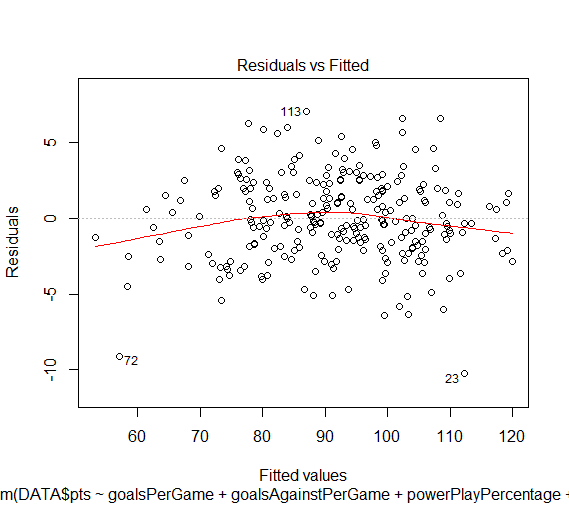
\includegraphics[width=0.7\linewidth]{AIC1}
	\caption{Residuals vs Fitted Values for AIC}
	\label{fig:Residuals vs Fitted Values for AIC}
\end{figure}
\begin{figure}
	\centering
	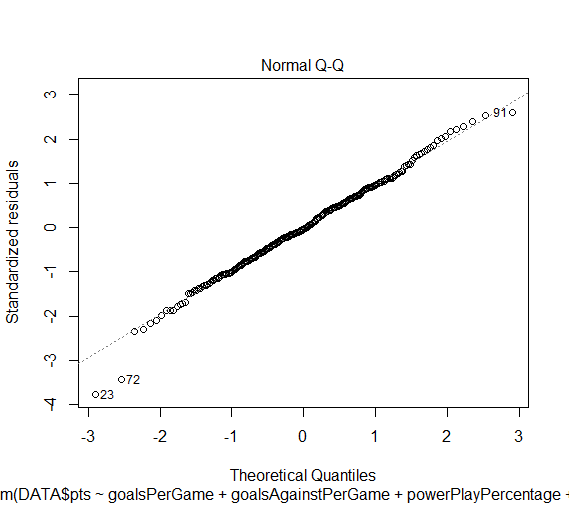
\includegraphics[width=0.7\linewidth]{AIC2}
	\caption{QQ Plot for AIC}
	\label{fig:QQ Plot for AIC}
\end{figure}
\begin{figure}
	\centering
	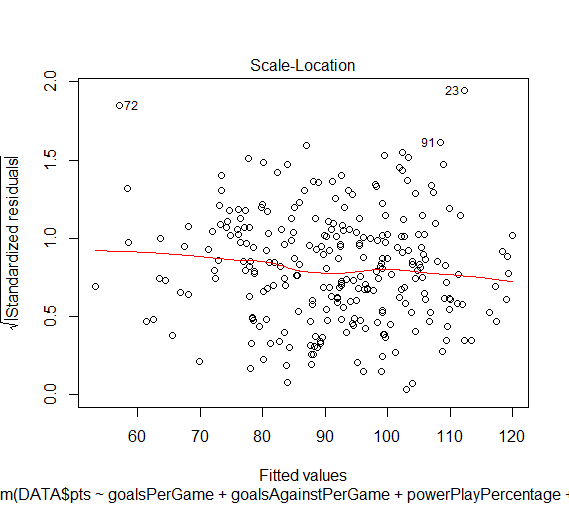
\includegraphics[width=0.7\linewidth]{AIC3}
	\caption{Scale-Location for AIC}
	\label{fig:Scale-Location for AIC}
\end{figure}
\begin{figure}
	\centering
	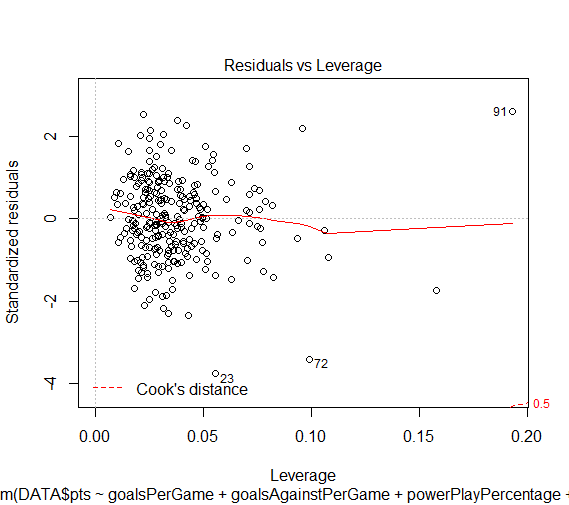
\includegraphics[width=0.7\linewidth]{AIC4}
	\caption{Residuals vs Leverage for AIC}
	\label{fig:Residuals vs Leverage for AIC}
\end{figure}
\begin{figure}
	\centering
	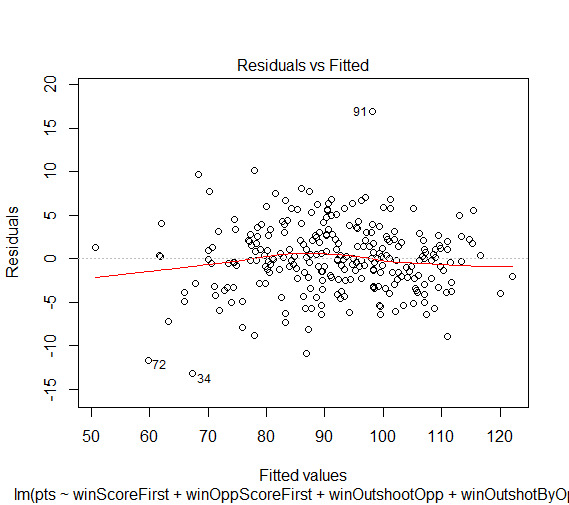
\includegraphics[width=0.7\linewidth]{R1}
	\caption{Residuals vs Fitted Values for R Squared}
	\label{fig:Residuals vs Fitted Values for R Squared}
\end{figure}
\begin{figure}
	\centering
	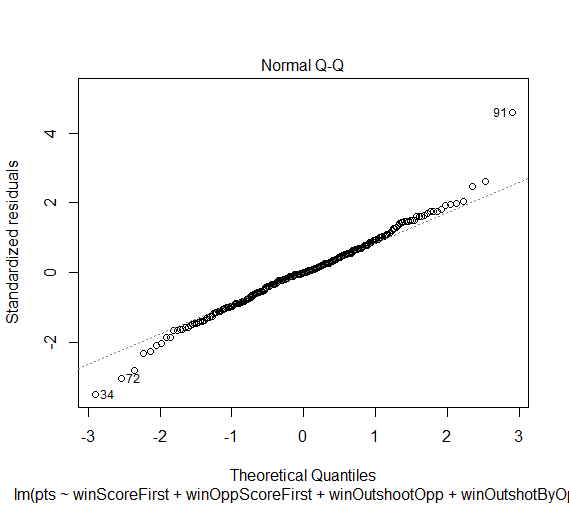
\includegraphics[width=0.7\linewidth]{R2}
	\caption{QQ Plot for R Squared}
	\label{fig:QQ Plot for R Squared}
\end{figure}
\begin{figure}
	\centering
	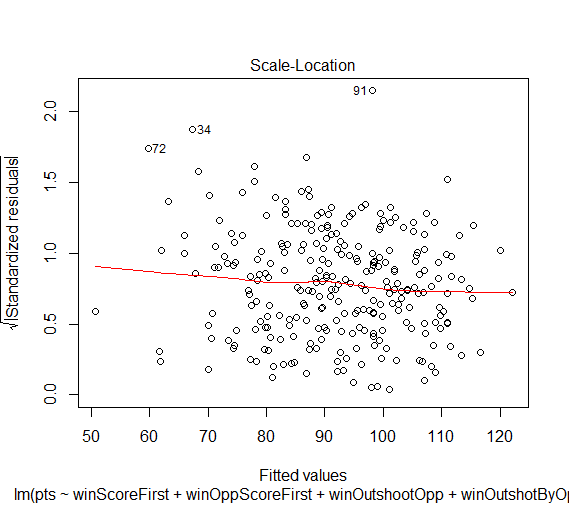
\includegraphics[width=0.7\linewidth]{R3}
	\caption{Scale-Location for R Squared}
	\label{fig:Scale-Location for R Squared}
\end{figure}
\begin{figure}
	\centering
	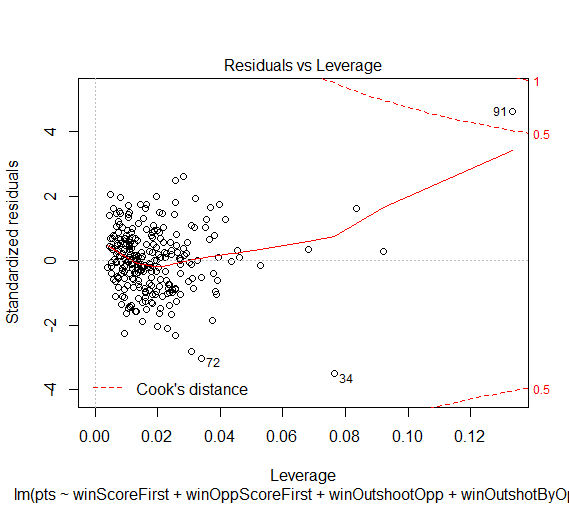
\includegraphics[width=0.7\linewidth]{R4}
	\caption{Residuals vs Leverage for R Squared}
	\label{fig:Residuals vs Leverage for R Squared}
\end{figure}




